\documentclass[aps,prl,onecolumn,groupedaddress,superscriptaddress]
{revtex4}

%=============================================================================
\usepackage{graphicx}
\usepackage{mathtools}
\usepackage{amssymb,latexsym}
\usepackage{amsmath,amsbsy}
\usepackage[dvipsnames]{xcolor} 

\newcommand{\lc}{\ensuremath{\Lambda_c}}
\newcommand{\fm}{\ensuremath{\,\text{fm}^{-1}}}
\newcommand{\abb}{\mbox{\ensuremath{A\oplus\,1}}}
\newcommand{\lec}{C^\Lambda}
\newcommand{\led}{D^\Lambda}
\newcommand{\eg}{\textit{e.g.}~}
\newcommand{\ie}{\textit{i.e.}~}
\newcommand{\eftnopi}{\mbox{EFT$(\not \! \pi)$}}
\newcommand{\ve}[1]{\ensuremath{\boldsymbol{#1}}}
\newcommand{\rms}[1]{\ensuremath{\langle r(#1)\rangle}}
\newcommand{\figref}[1]{fig.~\ref{#1}}
%=============================================================================

\begin{document}

\title{Stability of fermionic states with contact theories}
\author{M.~Sch{\"a}fer}\thanks{m.schafer@ujf.cas.cz}
\affiliation{Nuclear Physics Institute of the Czech Academy of Sciences, 25069 \v{R}e\v{z}, Czech Republic}
\affiliation{Czech Technical University in Prague, Faculty of Nuclear Sciences and Physical Engineering, B\v{r}ehov\'{a} 7, 11519 Prague 1, Czech Republic}
\author{L.~Contessi}\thanks{lorenzo.contessi@cea.fr}
\affiliation{Racah Institute of Physics, The Hebrew University, 91904 Jerusalem, 
Israel} 
\affiliation{AESNT, CEA, IRFU, D\'epartement de Physique Nucl\'eaire, Universit\'e de Paris Saclay, F-91191 Gif-sur-Yvette} 
\author{J. Kirscher}
\affiliation{Theoretical Physics Division, School of Physics and Astronomy,
The University of Manchester, Manchester, M13 9PL, United Kingdom} 
\date{\today}
%=============================================================================

\begin{abstract}
We analyze the stability of systems composed of isomassive fermions in which
the number of particles is larger than the number fermionic flavours. 
To this end, the leading order of a momentum- and flavour-independent
contact effective field theory is renormalized to shallow dimer and
trimer states.
The regulator dependence of the stability is assessed as a function
of particle number and of the proximity of the two-body interaction
to unitarity.
The systems become unstable
with respect to decays into spatially symmetric fragments
if the regulator-induced effective ranges
are below a certain threshold.
This critical range decreases when
the number of particles is increased 
down to a minimum range which is significantly
smaller than the dimer scale.
The closer the system is to unitarity, the
more particles are needed to attain the minimum. At unitarity, the
critical range tends to zero parabolically with the particle number.

We elaborate on the consequences of these results for the systematic
description of any system close to unitarity. For nuclei in particular,
the usefulness of the pionless theory
for the description of $P$-wave stable systems such as $^6$Li and $^7$Li effectively
is considered.
\end{abstract}

\maketitle

%=============================================================================
\vspace{4mm}
\paragraph*{Introduction}
If each particle of a set of $A$ isomassive fermions can be distinguished by an internal degree of
freedom, the dynamics changes significantly with this number $A$ exceeding the dimension $d$ of
the flavour space. For $A\leq d$, the system can realize bose-like behaviour in a totally
symmetric spatial state while mixed symmetry is demanded if $A>d$. 
If the mutual interaction is flavour independent, this change is solely a consequence
of the statistical properties of the particles.
As such, the difference between fermionic and bose-like few-body phenomena can be studied in a universal approach, which does not depend on the short-distance structure of the particle-particle interaction, namely, with a resonant contact interaction~\cite{1935RSPSA.148..146B}.
%
The ideal resonant system, {\it viz.} at unitarity, has
a two-body bound state exactly at the threshold with
a corresponding scattering length $a=\pm\infty$.
Physical systems typically deviate from this ideal. However, if
their two-body correlation/scattering length is much larger than any other relevant length scale of the problem, as a three-body extension, they  still share universal few-body phenomena, \eg~, the three-body Efimov effect~\cite{Efimov:1971zz}, the Tjon~\cite{tjon}~and Phillips~\cite{philli}~
correlations, and the spectrum of the multi-boson system~\cite{manybosons}.
Certain mesons, nuclei, and atoms~(see, \eg,
Refs.~\cite{Tornqvist:1991ks,Voloshin:2003nt,Braaten:2003he,philli,tjon,PhysRevLett.81.69})
are prominent members of this
universality class which exhibit structure at widely different scales.

With interactions of this type, three- and four-body systems driven by
fermionic substructures were also found in form of the absence of shallow
resonant~\cite{Kartavtsev_2007}~and bound states~\cite{Petrov:2005zz}~in
isomassive two-flavour three- and four-body systems, respectively.
It thus appears that the description of fermionic systems which exhibit
such peculiar structure, \eg, a hypothetical three-neutron (${}^3n$) resonance, 
needs to consider an additional scale which relaxes unitarity.
Multiple mechanisms could, in principle, generate such a scale:
a specific realization of the discrete scale invariance in the three-boson~\cite{Bedaque:1998kg}~
system with a $S$-wave three-body contact;
finite two-body scales beyond the scattering length;
the difference between particle number and flavour-space dimension ($A-d$); the absolute numbers of $A$, and $d$, respectively.

Here, we explore these possibilities with an effective field theory (EFT)
applied to a variety of few-body problems. 
This entails renormalization as a systematic way to trace the effect of
short-distance scales in a range of $A$-body observables for various flavour-space dimensions.

%=============================================================================
\vspace{4mm}
%\paragraph*{Theoretical framework}
\paragraph*{Theory}
The 
%development of a
minimal EFT for non-relativistic point particles exhibiting two- and three-body shallow states has been studied extensively
(\eg~Refs.\cite{Lepage:1997cs,vanKolck:1999mw, Bedaque:1998kg, Braaten:2004rn, Hammer:2017tjm, Hammer:2019poc}).
The theory is defined as a perturbative series and can be refined
systematically to attain a desired accuracy. Its Hamiltonian formulation at
leading order (LO) comprises zero-range two- and three-body vertices which
depend on the renormalization parameter~$\Lambda$:

\begin{align}
H = - \sum_{i<j} \frac{\hbar^2}{2m}\ve{\nabla}_{ij}^2+ \lec \sum_{i<j}{\delta_\Lambda(\ve{r}_i-\ve{r}_j)} 
\,+\nonumber\\
\led \sum_{ i<j<k \atop \text{cyc} }\delta_\Lambda(\ve{r}_i-\ve{r}_j)\delta_\Lambda(\ve{r}_i-\ve{r}_k).
\label{eq:hamiltonian}
\end{align}

In the expansion of any resultant amplitude, the LO is represented by all Born
terms depending solely on the coupling constants $\lec$ and $\led$. 
Parameters representing the aforementioned refinements
enter perturbatively at the order given na\"ively by their mass
dimension. 
In this work, a Gaussian regulator 
\mbox{$\delta_\Lambda(\ve{x}) \propto\Lambda^3 e^{-\frac{\Lambda^2}{4}\ve{x}^2}$} is used.
It induces a $\Lambda$ dependence in $\lec$ and $\led$ which was calibrated to
the energy of a single bound state in the two- ($B(2)$) and three-body
($B(3)$) system, respectively.
Whether or not the $\Lambda$ convergence of another amplitude depends on the
specific choice for $B(2)$ and $B(3)$ classifies the corresponding observable as
universal or emergent.
The few-body problem is thereby specified with five parameters: the particle's mass
(here, $m=938~$MeV), the number of particles ($A$) and flavours ($d$),
and the dimer and trimer binding energies.

We use this structure to consider a class of few-body systems with \abb~statistics
\footnote{We refer to a system of $A$ $d$-flavour fermions with $A>d$
as $d^p \oplus\,b$ with $p$ $d$-uplets of fermions which can share the same
spatial quantum states, and $b<d$ are the residual
particles which are not enough to fill the flavour degeneracy of the states.
This notation exposes the number of particles not on-shell
for the Pauli interaction.
For example, in this notation the nuclear $^6$Li is denoted $4 \oplus\,2$;
a hypothetical system of 33 atoms of Helium-3 (spin $1/2$ fermions),
$2^{16} \oplus\, 1$;}
as they approach the unitarity limit by
increasing the ratio
\mbox{$\upsilon:=B(3)/B(2)$}.
We choose the combinations $B(2)=1$~MeV with $B(3)\in\lbrace1.5$~\footnote{This constraint changes the
threshold structure significantly. Consequently, the ground states of \abb~systems are not expected in the
same $L_\text{total}=1$ channels. Consistently, our SVM calculations
do not yield bound states for this choice of $B(3)$.}$,\,3,\,4\rbrace$~MeV;
and $B(2)=0^+$ with $B(3)=3$~MeV.
Finally, the nuclear pionless EFT (\eftnopi) is renormalized to yield the
deuteron and triton binding energies of $B(2)=2.22$~MeV
and $B(3)=8.48$~MeV, respectively. 
The necessary fits for $\led$ employ Stochastic-Variational~(SVM,~\cite{Suzuki:1631377})~and
Resonating-Group~(RGM,~\cite{PhysRev.52.1083})~variational diagonalizations. $\lec$ is
determined via a Numerov-type integration of the appropriate one-dimensional
radial Schr\"odinger equation.

\vspace{4mm}
\paragraph*{Results}
%
\begin{figure}
    \centering
        \centering
        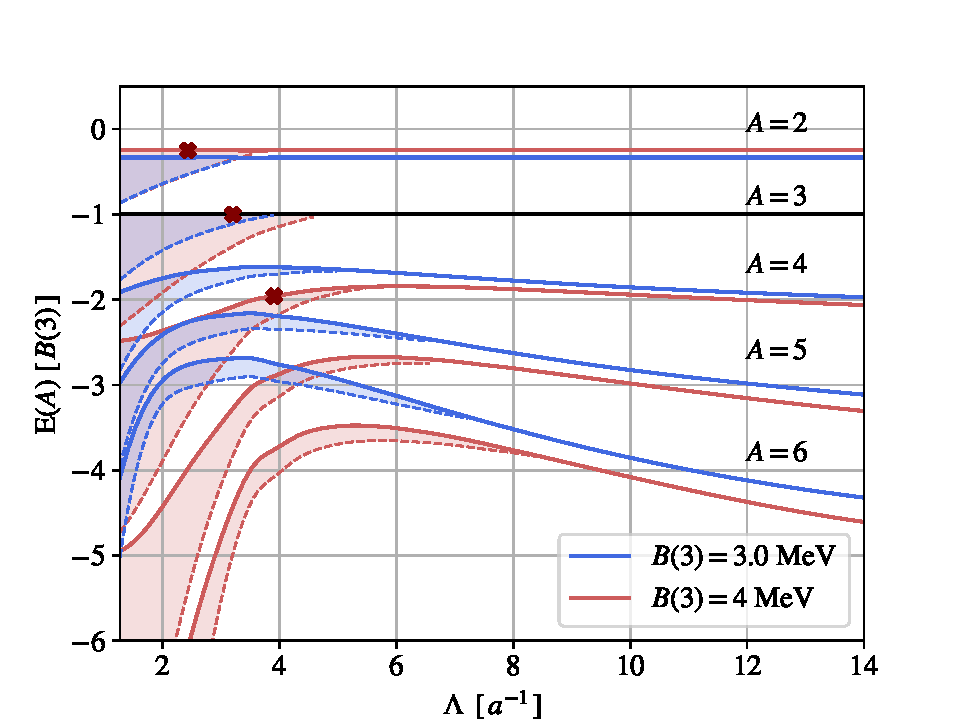
\includegraphics[width=\linewidth]{./p-systems-vs-l} 
        \caption{(Color online) LO Cutoff dependence of ground-state energies of $A$ bosons (solid) and \abb~mixed-symmetry systems
        (dashed) obtained with $B(2)=1~$MeV and $B(3)=3$ and $4~$MeV (blue and red) from \eqref{eq:hamiltonian}. With scattering volume set to zero, 
        the \abb~systems destabilize at smaller \lc~(red crosses, $B(3)=4$~MeV).}
        \label{fig:threshold}
\end{figure} 
%
The bose-like ground states of a theory with Hamiltonian of type \eqref{eq:hamiltonian}
have been analysed in detail numerically
(see \eg~Refs.\cite{Bazak:2016wxm,2015PhRvA..92c3626Y,Gattobigio:2012tk,vonStecher:2011zz,Gattobigio:2011ey}).
The SVM-predicted bose-like ground state energies for $A<7$ are shown in \figref{fig:threshold}. 
We find convergent behaviour as $\Lambda\to\infty$%~\footnote{In this work, we consider cutoffs $\Lambda$ up to $60\,a^{-1}$.}
~(renormalization-group (RG) invariance). At unitarity, we find the ratio $B(4)/B(3)$ consistent with
Refs.~\cite{Hammer:2006ct,2009NatPh...5..417V}.
In addition, we find
\mbox{$B(A)/B(3)\Big\vert_{\upsilon=3}<B(A)/B(3)\Big\vert_{\upsilon=4}$}
which implies that the universal ratios
$B(A)/B(3)$ are approached from below when taking the unitarity limit.

Now, we extend the analysis to \abb~systems.
In those, our SVM calculations with anti-symmetric wave function and
total orbital angular momentum $L_\text{total}=0$ yield no stable states, which confirms the intuitive demand for mixed spatial symmetry.
Even if expected due to Pauli repulsion, this result is non-trivial
because of the numerous angular couplings between particles
in many-fermion systems.

When projecting the spatial component of the variational basis onto
\mbox{$L_\text{total}=1$}, we find
\abb~systems for $A$
between 2 and 6 to sustain stable states \mbox{($B(\abb)>B(A)$)} for
$\Lambda\approx0.1\fm$.
In order to assess the universal character of these bound states, we vary the
cutoff 
($1.2~a^{-1}<\Lambda<60~a^{-1}$)
%($0.1<\Lambda<10$~fm$^{-1}$)
for all considered $\upsilon<\infty$.
Increasing the cutoff, \ie, decreasing the interaction range
while approaching the 
contact limit, unbinds the \abb~systems at some critical value $\lc$
(\figref{fig:threshold}).
\begin{figure}
\centering
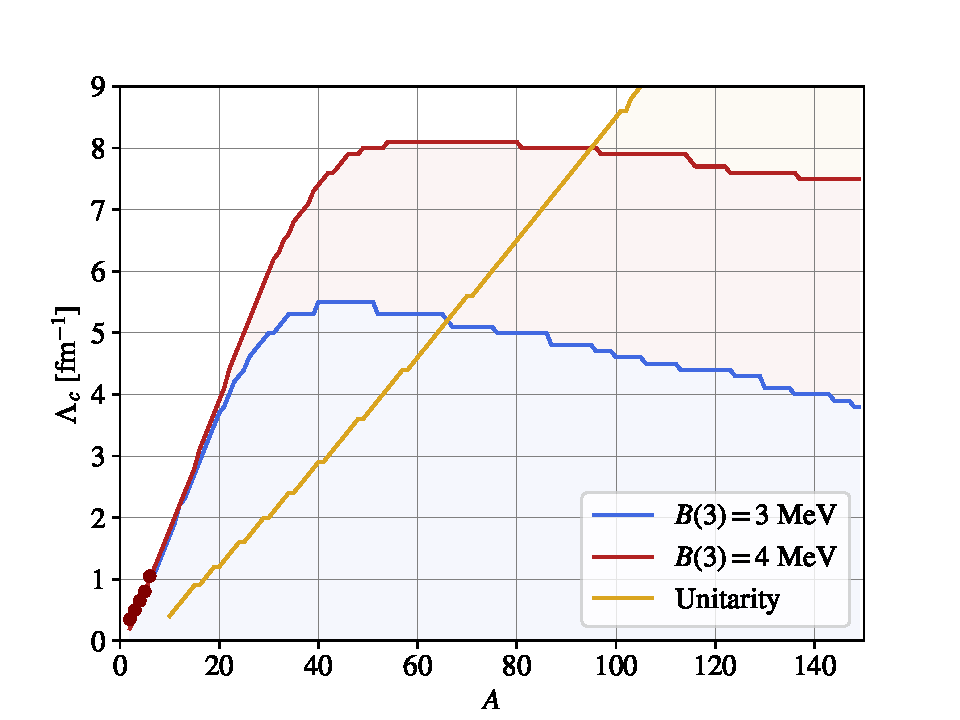
\includegraphics[width=\linewidth]{./RGM.pdf} 
\caption{(Color online) Dependence of the critical cutoff $\lc$ on the number of core particles
$A$. SVM few-body results are shown for $A<7$ (dots, $B(3)=4~$MeV) along with single-channel resonating-group approximations for $A<150$ (lines). The unitarity limit
(yellow) was realized with $B(2)\to0^+$ and $B(3)=3~$MeV and deviations from it
with $B(2)=1~$MeV and $B(3)\in\lbrace3,4\rbrace~$MeV (blue, red). 
In the shaded regions, the respective theories do sustain bound \abb~states,
while systems above the lines are unstable.
The step-like change in the curves results from a numerical criterion for the onset of binding and
can be removed systematically.}
\label{fig:RGM}
\end{figure}
%
%
The interaction range at which an \abb~system disintegrates
decreases with the number of particles $A=d$ comprising its
spatially symmetric core. For small systems, this relation is
almost linear, $\lc\propto A<7$.
To assess the dependence for $A>6$, we
employ a single-channel effective two-fragments resonating-group local
approximation (to be detailed in upcoming communication in extension of
Refs.~\cite{PhysRev.52.1083,Naidon_2016}). 
This approximation turns the few-body into a two-body problem
between a ``frozen'' core and the one residual particle which is forced out
of the Pauli shell.
The halo character of the problem motivates a one-parameter representation of 
the bose core as a product of harmonic oscillator
ground states because of
the increasingly large gap between $B(A)$ and $B(A-1)$ which does not
allow for its excitation by the out-of-shell
particle.
For $A<7$, the parameter is fitted to the SVM results for the rms radius of the core.
For larger $A$, we match the core wave function with the drop model
formula $r_\text{rms}\propto A^{1/3}$ as successfully employed in Ref.~\cite{manybosons}.
%    
Thereby, we find $\lc$ to increase up to a maximum number of particles $A^*$.
Both, $A^*$ and the associated $\lc(A^*)$ increase with $\upsilon$
(compare maxima of the two curves in \figref{fig:RGM}) and
we observe $\lim_{\upsilon\to\infty}A^*>100$.
The existence of $A^*$ thus appears to be an artifact of
the deviation from unitarity.
As a finite $\lc$ indicates a drastic change of the system's
behaviour, its magnitude being of the order of or even above a conceivable breakdown scale
would exclude this behaviour from the range of applicability of the theory.
For systems with breakdown scales below $\lc$, our results
expose the instability of \abb~system as universal.



\begin{figure}
\centering
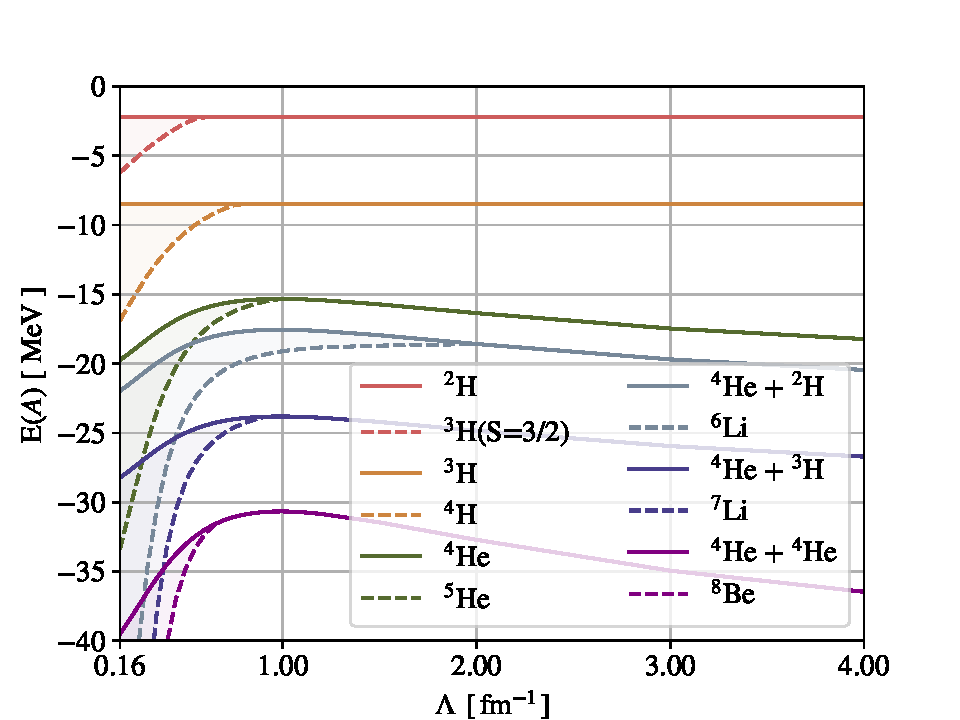
\includegraphics[width=\linewidth]{./Nuclear.pdf} 
\caption{(Color online) Cutoff dependence of nuclear ground-state energies
obtained in LO~\eftnopi. For $A<5$, solid lines represent nuclei with
spatially symmetric ground-state wave functions. For $A>4$,
solid lines mark the lowest decay threshold into two bose-like fragments.}
\label{fig:nuclear}
\end{figure}

To substantiate the conjecture of such a universal instability 
for nuclei and a more generic Pauli-shell structure,
we fit the experimental deuteron and triton binding energies,
$B(2)=2.22$~MeV and \mbox{$B(3)=8.48$}~MeV, respectively, 
thereby realizing a $SU(4)$-symmetric version of \eftnopi~\cite{Konig:2016utl}.
For $A\le 4$, we observe an instability pattern qualitatively identical to
those found earlier (compare \figref{fig:threshold} with \figref{fig:nuclear}).
Hence, the three-parameter theory predicts correctly the experimentally
established instability of nuclei in the
$^3\text{H}(\frac{3}{2}^-),\,^3n,\,^4\text{H},\,^{3,4}\text{Li},\,\text{and}~^5\text{He}$ channels.
In contrast, the isotopes $^{6,7}\text{Li}$ with $J^\pi=1^+$ and $\frac{3}{2}^-$,respectively,
are known to sustain bound states.
In these channels, we find particle-stable systems ($4\oplus\, 2$ and $4\oplus\,3$)
only below critical cutoffs $\lc\approx2\fm$ and $1\fm$.
For larger $\Lambda$, the systems break into an
$\alpha$-particle and a deuteron or triton, respectively.
Furthermore, we find $^8$Be ($4^2\oplus\, 0$, $J^\pi=0^+$), which is considered to be
stable without Coulomb repulsion~\cite{AFZAL:1969zz,Higa:2008dn},
to $\alpha$-decay at a $\lc\approx 0.7\fm\approx\mathcal{O}(m_{\pi})$.
$\lc$ being of the same order as the nuclear breakdown scale renders
the stability as a cutoff artifact.
We explain the loss of stability with increasing number of particles in
different Pauli shells heuristically
with the smaller spatial extent of the pertinent nuclear
fragments, \ie, the $\alpha$ particle, the triton, and the deuteron.
The larger is the rms radius of the fragment, the larger is its overlap with
the symmetric $\alpha$ core, which increases the attraction between the two.
Furthermore, our three-parameter calculations at $\Lambda<\lc$, \ie, when a stable
ground state is realized, postdict the ordering of states in the rotational spectrum
in $\rm ^8Be$ - $0^+$, $2^+$, and $4^+$ correctly. More specifically,
these states emerge in form of bound excited states for $\Lambda<0.4~{\rm fm^{-1}}$.

The study of the trajectories of the
bound-state poles through the respective $\alpha-\text{n}$, $\alpha-{}^2\text{H}$, $\alpha-{}^3\text{H}$, and $\alpha-\alpha$
thresholds at $\Lambda > \lc$
is crucial for the usefulness of \eftnopi~for the
description of these nuclear channels.
This will tell whether a perturbative insertion of subleading
order must move a shallow scattering pole to a stable one, or if
a non-perturbative mechanism has to account for the creation of the
pole anew. 
At unitarity, a shallow $2\oplus\,1$ pole cannot be fixed to a specific energy.
In this limit, \ie, without any scale, the resonance can only converge to threshold
or diverge to infinity for $\Lambda\to\infty$
\footnote{We thank U.~van~Kolck for clarifying discussions on this issue.}.
In the first case, three-body unitarity would be a universal consequence of the resonant two-body
interaction. In the second case, the pole is an unphysical artifact which disappears with the regulator.
In contrast, for $d>2$, scale invariance is broken, and the associated emergence of a
scale could pin the resonance to a finite energy.
As of now, such a study has not been done.

%To this end, we apply the method of analytical continuation of the coupling constant (ACCC, \eg,~Ref.~\cite{Kukulin_1977}) to the \abb~case.
%At unitarity, the resonant pole cannot be fixed to a specific energy as a consequence of
%scale invariance. In this absense of scales, the resonance can only only converge to threshold or diverge to infinity for $\Lambda\to\infty$.
%In the first case, three-body unitarity would be a universal consequence of the resonant two-body interaction. 
%In the second, the pole is an unphysical artifact which disappears with the regulator.
%Thereby, an attractive auxiliary three-body contact term is introduced with strength $\Delta^\Lambda$ structuraly identical to the one renormalizing the bosonic three-body system in \eqref{eq:hamiltonian}. 
%For a range of cutoffs (see \figref{fig:poletrajectory}), the initial $\Delta^\Lambda$ was chosen to bind the $2+1$ system before taking the limit $\Delta^\Lambda\to 0$ while following the bound state pole on its way on the physical (energy) sheet through the branch cut.
%After this transition (hatched area in \figref{fig:poletrajectory}), it represents a resonance.
%The pole remains on this sheet for $\Lambda\lesssim4\fm$. 
%For larger cutoffs, the pole passes through another branch cut and leaves the first unphysical sheet. 
%Thus, it is no longer a dimer-particle resonance. 
%Furthermore, its trajectory exhibits no convergent behaviour.
%An analogue of the dynamical pole generated (non-perturbatively) by the contact theory \eqref{eq:hamiltonian} in the two- and three-boson systems does not seem to exist in \abb~neither as a bound nor resonant state.


%\begin{figure}[h] 
%\centering 
%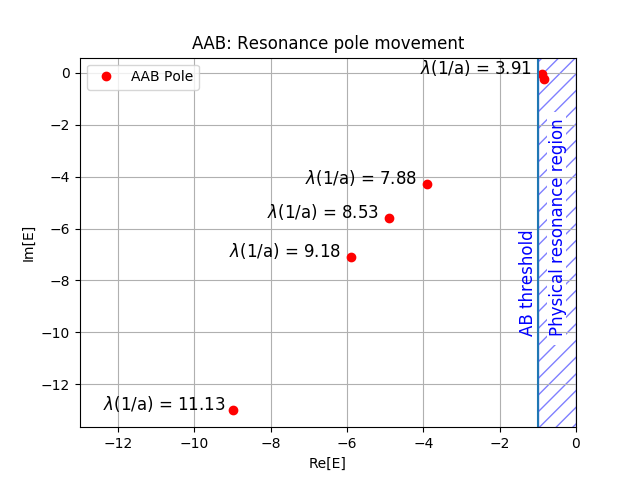
\includegraphics[width=0.8\textwidth]{./AAB_resonance_run.png} 
%\caption{Lowest Hamiltonian eigenvalue analytically continued below the lowest two-/three-fragment breakup (ordinate/vertical at Re$[E]=-1~$MeV) threshold for a $2+1$ system. Eigenvalues in the hatched region correspond to resonances which disappear with increasing regulator cutoff ($\lambda$ label) through the three-fragment breakup branch cut.} 
%\label{fig:poletrajectory}
%\end{figure}

For the conception of an extension of the \eftnopi~which predicts also the
particle-stable character of $^{6,7}$Li and $^8$Be in the zero-range limit,
we analyze the mechanism behind the stability of these systems for $\Lambda<\lc$.
Of all artifacts introduced by the finite range of the regulated contact interaction,
the finite effective range in the two-body $S$-wave channel
and a non-zero attractive two-body $P$-wave interaction are expected to dominate. 
Both contribute to the attraction in the \abb~system but their relative significance
in this role is obscure.
In other words, the finite-range interaction does not only describe a finite
but large $S$-wave scattering length but also other finite parameters of the
effective-range expansion of the $S$-wave amplitude like the effective range $r_0$. 
Furthermore, the scattering volume $a_1$ of the two-nucleon $P$-wave amplitude is non-zero as well.
To shed light on their
relative importance, we project the two-body interaction in an asymmetric internal state.
This forces two interacting particles into an even spatial state ($L=0,2,..$) 
removing any spatially asymmetric contributions. 
In effect, a reduction of $\lc^A$ by about $50\%$ is observed 
(crosses in \figref{fig:threshold}).
Hence, the finite $r_0$ and $a_1$ seem to be of similar significance for the stability
of the corresponding nuclear systems.




\vspace{4mm}
\paragraph*{Conclusion}
We find that a non-relativistic system
of $d+1$ particles with identical masses and a $d$-dimensional internal
flavour space cannot sustain a stable state if its dynamics is constrained
by representations of two- and three-body momentum-independent contact
interactions which are renormalized to yield a resonant two-body state
and a single bound three-body state and whose residual finite-range is
below a critical value. 
If the range of the regulated contact interactions, however,
surpasses the critical range, the $L_{\text{\scriptsize total}} = 1$
ground state of the $d+1$ particles is stable with respect to breakup
into a spatially symmetric $d$-body ground state and a single free particle.
This critical range decreases with the system's particle number increasing as $A=d+1$.
For a set of interactions close to unitarity, the critical range
reaches a minimum at a certain number of particles.
At unitarity, we observe that the critical range keeps decreasing up to $d\sim100$~particles.
Similarly, with the pionless EFT at leading order, we find the nuclear systems ${}^{6,7}$Li, and $^8$Be unstable, contrary to expectations. 

We investigate the finite effective-range and scattering volume of two bodies 
as the dominant parameters affecting stability. 
Both were found of similar importance to bind the studied systems at small cut-off.
With the vanishing of these parameters in the contact limit,
the result questions the capability of such theories for the description of $P$-wave-stable states
and asks for a study of the renormalization-group running of hypothetical shallow scattering poles. 
Only RG-stable poles might be stabilized with insertions of sub-leading operators,
while in their absence they would have to be created anew.
The latter result would have fundamental consequences for the effective-field-theory formulation.

\paragraph*{Acknowledgments}
We thank N.~Barnea,  M.~Birse, U.~van Kolck, J.~Mare\v{s}, N.~Walet for insightful
discussions.
M.S. was supported by the Czech Science Foundation GACR Grant No.19-19640S.
L.C. and J.K. acknowledge support from ``Espace de Structure et de r\'eactions
Nucl\'eaire Th\'eorique''  (ESNT, http://esnt.cea.fr )  at CEA-Saclay, where this work
was partially carried out.
L.C. was also supported by the Pazy Foundation and by the
Israel Science Foundation Grant No. 1308/16.

%=============================================================================

\bibliographystyle{ieeetr}
\bibliography{Thebibliography.bib}
\end{document}
